

%----------------------------------------------------------------------------------------
%	PACKAGES AND DOCUMENT CONFIGURATIONS
%----------------------------------------------------------------------------------------

\documentclass[a4paper,12pt]{article}
\usepackage[margin=1in]{geometry}
\renewcommand{\baselinestretch}{1.2}
\usepackage{siunitx} % Provides the \SI{}{} and \si{} command for typesetting SI units
\usepackage{graphicx} % Required for the inclusion of images
\usepackage{subfigure}
\usepackage{multirow}
\usepackage{amsmath} % Required for some math elements 
\usepackage{indentfirst}
\usepackage{times} % Uncomment to use the Times New Roman font
\usepackage{appendix}
\usepackage{verbatim}
\renewcommand{\multirowsetup}{\centering}  


%----------------------------------------------------------------------------------------
%	DOCUMENT INFORMATION
%----------------------------------------------------------------------------------------

\title{\rule{\textwidth}{0.3mm} \\UM–SJTU JOINT INSTITUTE \\ PHYSICS LABORATORY \\ (VP241) \\ \rule{\textwidth}{0.3mm} \\ [30 mm]  \Large{Laboratory Report} \\[5 mm]  Exercise 4 \\[1 mm] 
Polarization of Light \\[20 mm]} % Title
\author{Cao Zhiyuan} % Author name
\date{\today} % Date for the report

\begin{document}
\scshape

\maketitle % Insert the title, author and date

\begin{center}
\begin{tabular}{l l l}
\\[5 mm]
Partners:  \\
Name: Cao Zhiyuan & ID: 518370910030 & Group: 19 \\
Name: Gu Zheng & ID: 518370910190 & Group: 19 \\
~\\
Date Performed:\\
October 25, 2019\\
\end{tabular}
\end{center}

\thispagestyle{empty}


\newpage


\small\tableofcontents
\thispagestyle{empty}


\newpage

%----------------------------------------------------------------------------------------
%	SECTION 1
%----------------------------------------------------------------------------------------
\setcounter{page}{1}
\upshape
\section{\textsc{Objective}}
\begin{itemize}
\item Understand the basic properties of light, mainly the polarization phenomenon of light.
\item Learn and verify Malus' law.
\item Understand the roles half-wave and quarter-wave plates play in the optical systems.
\item Investigate on how to generate and detect the circularly and elliptically polarized light.
\end{itemize}

%----------------------------------------------------------------------------------------
%	SECTION 2
%----------------------------------------------------------------------------------------
\section{\textsc{Theoretical background}}
In our nature, waves exists everywhere. Generally speaking, waves can be classified into longitudinal and transverse wave based on the direction of oscillations. As for light, which can be described in terms of electromagnetic waves, since its plane of oscillations of the electric field vector is perpendicular to the direction of light propagation, light can be regarded as transverse wave. 
\par On of the most important characteristics of transverse wave is the polarization phenomenon. In this lab, we focus on the polarization of light. The commonest light in our life is \textit{natural light}, which is also called \emph{unpolarized light}. For natural light, the incident light is a random mixture of waves with the electric field vector oscillating in all possible transverse directions. Also, the distribution of the electric field vector if uniform in all directions. On the other hand, for \textit{polarized light} the distribution of directions is not uniform. Starting from these basics theories, research on wave polarization has a numerical application in the real world, ranging from optical measurement devices, to the realm of crystal structure.

\subsection{\textsc{Polarization of light}}
The electric field vector $\vec{E}$ corresponds to the visible part of the spectrum in the context of electromagnetic waves and is sometimes called the light vector. It describes an propagating electric field that changes with time. In the plane perpendicular to the propagation direction of the wave, the direction of the light vector may be different. The light whose light vector maintains a certain direction of oscillation is called \textit{linear polarization}, and the axis that defines the direction is called the polarization axis. (Fig.1)

\begin{figure}[h] 
    \centering
    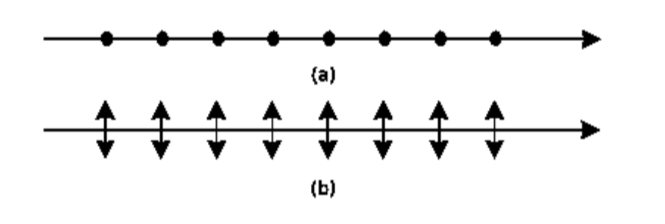
\includegraphics[width=0.9\textwidth]{Fig1} 
    \caption{(a) Linearly polarized light with the polarization axis perpendicular to the page plane. (b) Linearly polarized light with the polarization axis parallel to the page plane. \cite{labmanual}} 
\end{figure}

There are other types of polarized light. For \textit{circularly polarized light}, the direction of the light vector and the direction of the light propagation rotate so that the end point moves in a circular motion. For \textit{circularly polarized light}, the end point of direction moves along an ellipse. The Figure is shown in Fig.2.

\begin{figure}[h] 
    \centering
    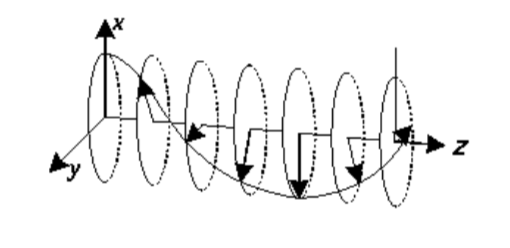
\includegraphics[width=0.6\textwidth]{Fig2} 
    \caption{Elliptically polarized light propagating in the z direction. The light is polarized in the xy plane. \cite{labmanual}} 
\end{figure}

Although unpolarized light is emitted from ordinary light sources, it can be regarded as a mixture of linearly polarized light whose distribution of direction is statistically equal to each other. For partially polarized light, it can be seen as combining a natural light and a polarized light together, because a partial polarized light has a non-uniform distribution of directions of light vector, indicating it can be decomposed into a natural light and a polarized one.

\subsection{\textsc{Polarizer}}
The device we commonly used to produce polarized light is called polarizer, which can also be called polaroid. According to the principle of dichroism, a selective absorption mechanism tends to allow the light polarized in a certain direction (direction of the crystal alignment) to pass through the material, while the light polarized in all other directions is absorbed \cite{labmanual}. A polarizer is able to transform an incident light which is originally natural into linearly polarized light.

\par Not only does a polarization device transform natural light into polarized light (the function of a polarizer), but it also act as a device to analyze different polarized light. In this case, polarizer acts as an analyzer.  

\subsection{\textsc{Malus' law}}
After the light passes through a polarization device, one noticeable effect is that the intensity of light brightness changes, and the light may become darker.

\begin{figure}[h] 
    \centering
    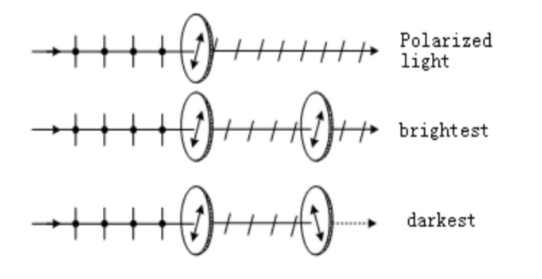
\includegraphics[width=0.6\textwidth]{Fig3} 
    \caption{Change in the brightness of the light depends on the mutual orientation of the polarizer and the analyzer. \cite{labmanual}} 
\end{figure}

Assume that two polarization device are places together in a line (See Fig.3), where the left one acts as a polarizer and the right one acts as an analyzer, and given that the angle between their polarization axes is $\theta$, the intensity of the light leaving the anlayzer is:
\begin{equation}
I_{light} = I_{light,0} cos^2\theta
\end{equation}
where $I_{light}$ is the intensity of light passing through the polarizer, and $I_{light,0}$ is the intensity of light passing through the analyzer. Equation (1), discovered in 1809, is known as the Malus’ law, which is named after Etienne-Louis Malus.

\par From the equation, we can clearly observe that if there is a single polarizer, the transmitted light intensity of an incident polarized light will change periodically when the polarizer is rotated, with a period $T = 2\pi$. For different type of polarized light, the phenomenon will also differer from each other:
\begin{itemize}
\item For an initially partially or elliptically polarized incident light, the minimum intensity will not reaches zero because of the geometric shape of light vector distribution. 
\item For a natural or circularly polarized light, the intensity will not change at all.
\end{itemize}
Based on above properties, by using a polarizer, we can tell linearly polarized light from the natural and circularly polarized light ones.

\subsection{\textsc{Generation of Elliptically and Circularly Polarized Light. Half-wave and Quarter-wave Plates}}
Assume that a linearly polarized light passes thorough a crystal plate whose surface is generally parallel to the optical axis, and the angle between the polarization axis and the optical axis of the plate is $\alpha$. Then the linearly polarized light is decomposed into two different waves: one is e-wave whose oscillation direction is parallel to the optical axis of the plate while another is o-wave whose oscillation direction is perpendicular to the optical axis. They are named as extraordinary axis and ordinary axis respectively. In fact, the two waves propagate in the same direction, however, with a different speed. We can calculate the resulting optical path difference of a plate with thickness d as follows:
\begin{equation}
\Delta = (n_e - n_o) d
\end{equation}
Hence, we are able to find out the phase difference accordingly:
\begin{equation}
\displaystyle \delta = \frac{2\pi}{\lambda} (n_e - n_o) d
\end{equation}
where $\delta$ is the phase difference, $\lambda$ stands for the wavelength, $n_e$ refers to the refractive index for the extraordinary axis, and $n_o$ is the refractive index for the ordinary axis. A crystal with $\delta > 0$ is called positive crystal, while a $\delta > 0$ one is called negative crystal.

\begin{figure}[h] 
    \centering
    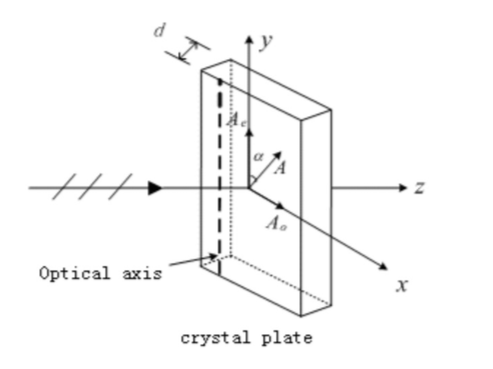
\includegraphics[width=0.6\textwidth]{Fig4} 
    \caption{Linearly polarized light passing through a waveplate. \cite{labmanual}} 
\end{figure}

In Fig.4, we can see that there are two components of light vectors, which can be expressed as follows:
\begin{center}
$E_x= A sin\alpha cos\omega t = A_o cos\omega t$\\
$E_y= A cos\alpha cos(\omega t+\delta) = A_e cos(\omega t+\delta)$
\end{center}

To obtain the trajectory of the light vector, we eliminate the time $t$ in the above equations, and we have:
\begin{equation}
\displaystyle \frac{E_x^2}{A_o^2} + \frac{E_y^2}{A_e^2} - 2\frac{E_x E_y}{A_o A_e} cos\delta = sin^2\delta
\end{equation}
Note that Eq.(4) is the only valid for $\delta = \pm \pi/2$.
\par For some particular chosen thickness of plate, the optical path will change at the same time, and some interesting cases occur, which is discussed below:
\begin{itemize}
\item If $\Delta = k \lambda$ (k = 0, 1, 2, ...), the phase difference $\delta = 0$. Eq.(4) can be rewritten into a simpler form:
	\begin{center}
	$ \displaystyle E_y = \frac{A_e}{A_o}E_x$ 
	\end{center}
which is actually a linear equation. So the transmitted light is linearly polarized and oscillates in the same direction. A wave plate satisfying this condition is called a \textit{full wave plate}. Light passing through a full-wave plate will not change its polarization state.

\item If $\Delta = (2k+1) \lambda/2$ (k = 0, 1, 2, ...), the phase difference $\delta = \pi$. Eq.(4) can be rewritten into a simpler form:
	\begin{center}
	$ \displaystyle E_y = -\frac{A_e}{A_o}E_x$ 
	\end{center}
Transmitted light is also linearly polarized with the polarization axis rotating $2\alpha$. A wave plate satisfying this condition is called a \textit{1/2 wave plate} or \textit{a half wave plate}. When the polarized light passes through the half-wave plate, the rotation angle of its polarization axis is $2\alpha$. Specifically, if $\alpha= \pi/4$, the transmitted light's polarization axis is vertical to that of the original light.

\item If $\Delta = (2k+1) \lambda/4$ (k = 0, 1, 2, ...), the phase difference $\delta = \pm \pi/2$. Eq.(4) can be rewritten into a simpler form:
	\begin{center}
	$ \displaystyle \frac{E_x^2}{A_o^2} + \frac{E_y^2}{A_e^2} = 1$ 
	\end{center}
As a result, the light is elliptically polarized. In this case, the very waveplate is called a \textit{1/4-wave plate} or a \textit{quarter-waveplate}, and is very important in optical experiments.
\end{itemize} 
Specially, if $A_e = A_o = A$, then we obtain $E_x^2 + E_y^2 = A^2$. As a result, the transmitted light is circularly polarized. The polarization state after the light passes through the wave plate will vary, depending on the different angle. The scenarios are listed in Table 1:

\begin{table}[h]
\begin{center}
\begin{tabular}{|c|c|c|}
\hline
$\alpha$ & state of the transmitted light & Polarization axis and the optical axis \\
\hline 
0 & linearly polarized & parallel \\
\hline
$\pi/2$ & linearly polarized & perpendicular \\
\hline
$\pi/4$ & circularly polarized & / \\
\hline
otherwise & elliptically polarize & / \\
\hline
\end{tabular}
\caption{Relationship between angle $\alpha$ and polarization state.}
\end{center}
\end{table}



%----------------------------------------------------------------------------------------
%	SECTION 3
%----------------------------------------------------------------------------------------
\section{\textsc{Apparatus and Experimental Setup}}
In this lab, we will use the following apparatus, which are placed on an optical bench:
\begin{itemize}
\item a semiconductor laser
\item a tungsten iodine lamp
\item a silicon photo-cell
\item a UT51 digital universal meter
\item two polarizers
\item 1/2-wave and 1/4–wave plates
\item a lens with a glass sheet
\end{itemize}

Then, the range or precision of the apparatus are listed in Table 2 below:

\begin{table}[h]
\begin{center}
\begin{tabular}{|c|c|}
\hline
 & Range/Precision \\
\hline
Angle & $ \pm 2^{\circ} $ \\
\hline
Current & $ \pm 0.001 \mu A $ \\
\hline
\end{tabular}
\caption{Range and precision of the apparatus.}
\end{center}
\end{table}



%----------------------------------------------------------------------------------------
%	SECTION 4
%----------------------------------------------------------------------------------------
\section{\textsc{Procedures \cite{labmanual}}}
\subsection{\textsc{Apparatus Adjustment}}
\begin{itemize}
\item[(1)] First, we adjust the photo-cell by choosing the appropriate aperture. In this experiment, we use only 6.0 aperture, because it preserves the incident light intensity (shown in Fig.5). Otherwise, the intensity of light may get reduced, resulting in a zero reading on the universal meter.
\begin{figure}[h] 
    \centering
    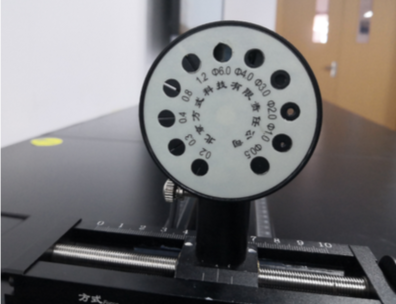
\includegraphics[width=0.6\textwidth]{Fig5} 
    \caption{Photo-cell. \cite{labmanual}} 
\end{figure}

\item[(2)] Second, with the laser fixed at one of the ends of the bench, we place the lens and the glass sheet in front of it. Then we make sure that the light passes through the center of the lens.

\item[(3)] Third, the distance between the lens and the laser is adjusted to the focal length of the lens.

\item[(4)] Forth, we move the glass sheet along the bench. If the size of the light spot on the glass varies significantly, repeat Step 2.

\item[(5)] Eventually, we remove the glass sheet, and set the digital universal meter in the appropriate mode and range.
\end{itemize}

\subsection{\textsc{Demonstration of Malus’ Law}}
In this section, since the light source we use has already been linearly polarized source. The method we use to verify Malus' Law has some difference than the normal one. Details are shown as follows:
\begin{itemize}
\item[(1)] First, we fix the analyzer and rotate the polarizer. We will discover that the intensity of light changes periodically. Then, we need to choose the position of the polarizer where the light intensity is maximum. In this way, the output linearly polarized light is "preserved" and has the original intensity.

\item[(2)] Second, we rotate the analyzer for 360$^{\circ}$ and observe a change in the light intensity to find the maximum electric current $I_0$. Then, we remain the position where the light intensity is maximum.

\item[(3)] Third, the angle of analyzer is 90$^{\circ}$. At this point, the polarizing axes of the polarizer and the analyzer are perpendicular to each other.

\item[(4)] Finally, we rotate the analyzer from 90$^{\circ}$ to 0$^{\circ}$ and record the magnitude of the current I every 5$^{\circ}$. Record the values in a table and plot the graph $I/I_0$ vs. $cos2 \theta$. After that, we perform linear fitting and compare the data with the theoretical result.
\end{itemize}

\subsection{\textsc{Linearly Polarized Light and the Half-wave Plate}}
\begin{itemize}
\item[(1)] We set up the equipment on the optical bench as shown in Fig.6. A is the analyzer and P is the polarizer. Set the polarizing axes of A and P perpendicular to each other before placing the 1/2-wave plate in the apparatus; extinction of the light can be observed on screen.

\item[(2)] After inserting the 1/2-wave plate, we rotate it to make the light extinction appear again and set this position as the initial position.

\item[(3)] We rotate the 1/2-wave plate for $\alpha = 10^{\circ}$ from the initial position and the light extinction will be broken. Then rotate A to make the light extinction appear again, record the angle of rotation $\Delta \theta$ in a table.

\item[(4)] Finally, we rotate the 1/2-wave plate for $10^{\circ}$ from the previous position (now $\alpha = 10^{\circ}$) and repeat Step 3. Repeat this step (increase $\alpha$) for 8 times. Plot the graph $\Delta \theta$ vs. $\theta$.

\begin{figure}[h] 
    \centering
    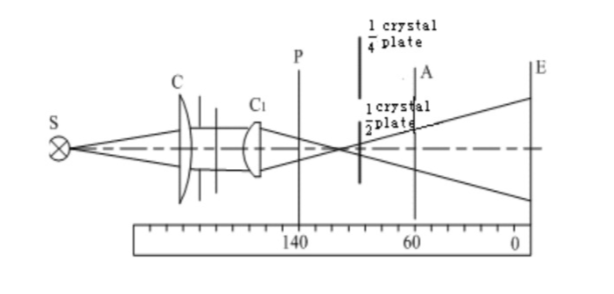
\includegraphics[width=0.7\textwidth]{Fig6} 
    \caption{Experimental setup for the 1/2-wave plate. \cite{labmanual}} 
\end{figure}

\end{itemize}

\subsection{\textsc{Circularly and Elliptically Polarized Light and the 1/4-wave Plate}}
\begin{itemize}
\item[(1)] First, we set up the equipment on the optical bench as shown in Fig.6, and set the polarizing axes of A and P perpendicular to each other before placing the 1/4-wave plate in the apparatus; extinction of the light can be observed on screen. At this point the angle $\theta = 90^{\circ}$.


\item[(2)] Second, after inserting the 1/4-wave plate, we rotate it to make the light extinction appear again and set this position as the initial position. At this point $\alpha = 0^{\circ}$. Rotate the 1/4-wave plate and observe the change in the light intensity.

\item[(3)] Third, we rotate the analyzer for $ 360^{\circ}$, and record the light intensity (which is indicated by the current I) for every $ 360^{\circ}$. Record the data in a table.

\item[(4)] We rotate the 1/4-wave plate for $ 20^{\circ}$, repeat Step 3.

\item[(5)] We rotate the 1/4-wave plate for $ 45^{\circ}$, repeat Step 3.

\item[(6)] After that, we rotate the 1/4-wave plate for $ 70^{\circ}$. Then rotate the analyzer and record its position and the magnitude of the current when the light intensity reaches a maximum.

\item[(7)] Then, we plot the relation between the rotation angle of the analyzer and the light amplitude in polar coordinates. Normalize the amplitude by its maximum value. Mark the position recorded in Step 6 and compare it with the data recorded in Step 4.

\item[(8)] Finally, we compare the result of Step 5 with that for the circular polarization. Plot a linear fit to the data when the angle is $ 45^{\circ}$.
\end{itemize}

%----------------------------------------------------------------------------------------
%	SECTION 5
%----------------------------------------------------------------------------------------
\section{\textsc{Results}}
\subsection{\textsc{Apparatus adjustment}}
According to what we have discussed in 4.1, we successfully adjust and warm up the apparatus we will use in this experiment.

\subsection{\textsc{Demonstration of Malus’ Law}}
In this section, we verify Malus' law, and the detailed results are shown in Table 3.

\newpage
Uncertainty of $\theta$ is $2^{\circ}$
\begin{table}[h]
\begin{center}
\begin{tabular}{|c|c||c|c|}
\hline
\multicolumn{4}{|c|}{Maximum Electric Current $I_0$ ~~~~~~~ $ 1.211 \pm 0.001 [\mu A]$} \\
\hline
$\theta$ & $I [\mu A] \pm 0.001 [\mu A]$ & $\theta$ & $I [\mu A] \pm 0.001 [\mu A]$ \\
\hline
$0^{\circ}$ & 1.211 & $50^{\circ}$ & 0.506\\
\hline
$5^{\circ}$ & 1.203 & $55^{\circ}$ & 0.423\\
\hline 
$10^{\circ}$ & 1.178 & $60^{\circ}$ & 0.320\\
\hline
$15^{\circ}$ & 1.122 & $65^{\circ}$ & 0.223\\
\hline
$20^{\circ}$ & 1.123 & $70^{\circ}$ & 0.154\\
\hline
$25^{\circ}$ & 1.056 & $75^{\circ}$ & 0.089\\
\hline
$30^{\circ}$ & 0.951 & $80^{\circ}$ & 0.041\\
\hline
$35^{\circ}$ & 0.855 & $85^{\circ}$ & 0.013\\
\hline
$40^{\circ}$ & 0.736 & $90^{\circ}$ & 0.000\\
\hline
$45^{\circ}$ & 0.620 &  &  \\
\hline
\end{tabular}
\caption{Measurement data of Malus' law demonstration.}
\end{center}
\end{table}

\begin{table}[h]
\begin{center}
\begin{tabular}{|c|c|c|c|c||c|c|c|c|c|}
\hline
$\theta$ & $I / I_0$ & $u_{I / I_0}$ & $cos^2\theta$ & $u_{cos^2\theta}$ & $\theta$ & $I / I_0$ &  $u_{I / I_0}$ & $cos^2\theta$ & $u_{cos^2\theta}$ \\
\hline
$0^{\circ}$ & 1.0000 & 0.0012 & 1 & 0 & $50^{\circ}$ & 0.4178 & 0.0009 & 0.41 & 0.03\\
\hline 
$5^{\circ}$ & 0.9934 & 0.0012 & 0.992 & 0.006 & $55^{\circ}$ & 0.3493 & 0.0009 & 0.33 & 0.03\\
\hline 
$10^{\circ}$ & 0.9727 & 0.0012 & 0.970 & 0.012 & $60^{\circ}$ & 0.2642 & 0.0009 & 0.25 & 0.03\\
\hline 
$15^{\circ}$ & 0.9265 & 0.0011 & 0.933 & 0.017 & $65^{\circ}$ & 0.1841 & 0.0008 & 0.18 & 0.03\\
\hline 
$20^{\circ}$ & 0.9273 & 0.0011 & 0.88 & 0.02 & $70^{\circ}$ & 0.1272 & 0.0008 & 0.12 & 0.02\\
\hline 
$25^{\circ}$ & 0.8720 & 0.0011 & 0.82 & 0.03 & $75^{\circ}$ & 0.0735 & 0.0008 & 0.067 & 0.017\\
\hline 
$30^{\circ}$ & 0.7853 & 0.0010 & 0.75 & 0.03 & $80^{\circ}$ & 0.0339 & 0.0008 & 0.030 & 0.012\\
\hline 
$35^{\circ}$ & 0.7060 & 0.0010 & 0.67 & 0.03 & $85^{\circ}$ & 0.0107 & 0.0008 & 0.008 & 0.006\\
\hline 
$40^{\circ}$ & 0.6078 & 0.0009 & 0.59 & 0.03 & $90^{\circ}$ & 0.0000 & 0.0008 & 0 & 0\\
\hline 
$45^{\circ}$ & 0.5120 & 0.0009 & 0.50 & 0.03 &  &  &  &  & \\
\hline 
\end{tabular}
\caption{Uncertainty of data of Malus' law demonstration.}
\end{center}
\end{table}

After calculations, we obtain the data in Table 4. For sample calculation, we choose the case when $\theta = 5^{\circ}$, where $I_0 = 1.211 \pm 0.001[\mu A]$ and $I = 1.203 \pm 0.001[\mu A]$. We will obtain:
\begin{center}
$\displaystyle \frac{I}{I_0} = \frac{1.203}{1.211} = 0.9934 \pm 0.0012$, ~~~ $\displaystyle r_{u_{\frac{I}{I_0}}} = 0.12 \%$
\end{center}
and 
\begin{center}
$\displaystyle cos^2\theta = cos^2 5^{\circ}= 0.992 \pm 0.006$, ~~~ $\displaystyle r_{u_{cos^2\theta}} = 0.6 \%$
\end{center}
Hence our relative error is small and acceptable. Detailed calculations regarding uncertainties are shown in Appendix A.

\par Then, with the help of Origin, we perform a linear fit, which is shown in Fig.7. 

\begin{figure}[h] 
    \centering
    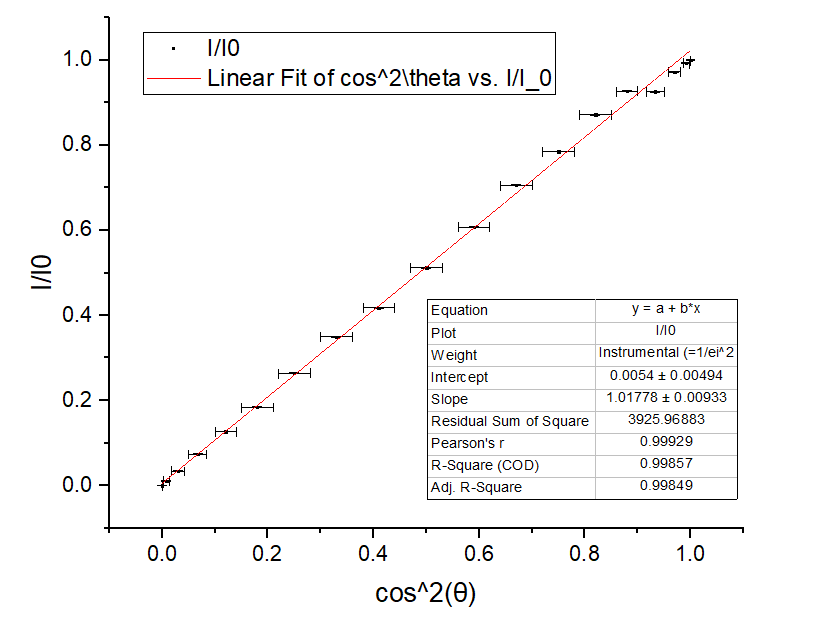
\includegraphics[width=0.7\textwidth]{R1} 
    \caption{Linear fit for $I/I_0~vs.~cos^2\theta$.} 
\end{figure}

From Fig.7, we can see that the value of Pearson's R equals to 0.99929, which is close to 1, demonstrating that $I/I_0$ and $cos^2\theta$ do have a linear relationship. Besides, since the slope is 1.01778, which is also close to 1, we obtain:
\begin{center}
$I/I_0 = cos^2\theta$
\end{center}
i.e., we have
\begin{center}
$I = I_0 cos^2\theta$
\end{center}
which matches the Malus' Law, with a relative uncertainty:
\begin{center}
$\displaystyle u_p = \frac{1.01778-1}{1} = 1.8\%$
\end{center}

\subsection{\textsc{Linearly Polarized Light and the Half-wave Plate}}
In this section, the data we recorded are shown in Table 4.

\begin{table}[h]
\begin{center}
\begin{tabular}{|c|c|}
\hline
Rotation angle of the 1/2-wave plate & Rotation angle of the analyzer [$^{\circ}$] $\pm$ 2 [$^{\circ}$] \\
\hline 
initial & 342 \\
\hline 
10$^{\circ}$ & 327 \\
\hline
20$^{\circ}$ & 296 \\
\hline
30$^{\circ}$ & 276 \\
\hline
40$^{\circ}$ & 259 \\
\hline
50$^{\circ}$ & 237 \\
\hline
60$^{\circ}$ & 217 \\
\hline
70$^{\circ}$ & 198 \\
\hline
80$^{\circ}$ & 178 \\
\hline
90$^{\circ}$ & 158 \\
\hline
\end{tabular}
\caption{Measurement data of Linearly Polarized Light and the Half-wave Plate.}
\end{center}
\end{table}

Then, we obtain the data with uncertainties, which is shown in Table 6.

\begin{table}[h]
\begin{center}
\begin{tabular}{|c|c|c|c|}
\hline
Rotation angle of & \multirow{2}{1cm}{$u_{\theta_1}$} & Rotation angle of & \multirow{2}{1cm}{$u_{\theta_2}$} \\ the 1/2-wave plate&  & the analyzer [$^{\circ}$] $\pm$ 2 [$^{\circ}$] & \\
\hline 
initial & 2$^{\circ}$ & 0 & 2$^{\circ}$\\
\hline 
10$^{\circ}$ & 2$^{\circ}$ & 15 & 3$^{\circ}$\\
\hline
20$^{\circ}$ & 2$^{\circ}$ & 46 & 3$^{\circ}$\\
\hline
30$^{\circ}$ & 2$^{\circ}$ & 66 & 3$^{\circ}$\\
\hline
40$^{\circ}$ & 2$^{\circ}$ & 83 & 3$^{\circ}$\\
\hline
50$^{\circ}$ & 2$^{\circ}$ & 105 & 3$^{\circ}$\\
\hline
60$^{\circ}$ & 2$^{\circ}$ & 125 & 3$^{\circ}$\\
\hline
70$^{\circ}$ & 2$^{\circ}$ & 144 & 3$^{\circ}$\\
\hline
80$^{\circ}$ & 2$^{\circ}$ & 164 & 3$^{\circ}$\\
\hline
90$^{\circ}$ & 2$^{\circ}$ & 184 & 3$^{\circ}$\\
\hline
\end{tabular}
\caption{Uncertainty of data of Linearly Polarized Light and the Half-wave Plate.}
\end{center}
\end{table}

\newpage
Now, we use Origin to perform a linear fit. The result is shown in Fig.8.
\begin{figure}[h] 
    \centering
    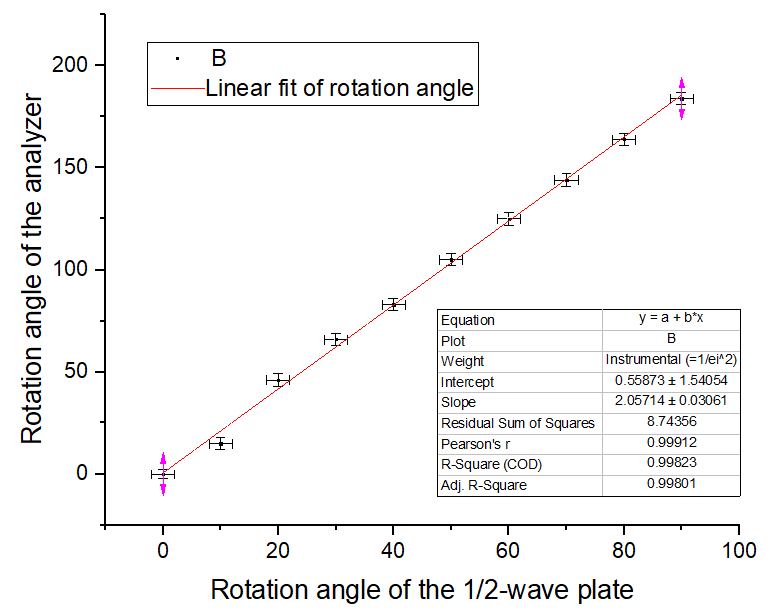
\includegraphics[width=0.7\textwidth]{R2} 
    \caption{Linear fit for rotation angle of the analyzer vs. 1/2-wave plate.} 
\end{figure}

From Fig.8, we can see that the value of Pearson's R equals to 0.99912, which is close to 1, demonstrating that $\theta_1$ and $\theta_2$ do have a linear relationship. Besides, since the slope is 2.06714, which is close to 2.Hence, we conclude that when a polarized light passes through a 1/2-wave plate, its polarization axis is rotated by $2\alpha$, with a relative uncertainty:
\begin{center}
$\displaystyle u_p = \frac{2.06714-2}{2} = 3\%$
\end{center}

\subsection{\textsc{Circularly and Elliptically Polarized Light and the 1/4-wave Plate}}
\subsubsection{\textsc{Rotation angle 0$^\circ$}}
In this section, the data is recorded in Table 7:

\begin{table}[h]
\begin{center}
\begin{tabular}{|c|c|c||c|c|c|}
\hline
\multicolumn{6}{|c|}{Rotation angle of 1/4-wave plate: $0^{\circ}$}\\
\hline 
\multicolumn{6}{|c|}{Maximum Electric Current $I_0$ ~~~ 1.452 $\pm$ 0.001$\mu A$}\\
\hline 
$\theta$ & $I [\mu A] \pm 0.001 [\mu A]$ & $\sqrt{\frac{I}{I_0}}$ & $\theta$ & $I [\mu A] \pm 0.001 [\mu A]$ & $\sqrt{\frac{I}{I_0}}$ \\
\hline
0$^{\circ}$ & 0.000 & 0 & 180$^{\circ}$ & 0.002 & 0.037 \\
\hline 
10$^{\circ}$ & 0.047 & 0.180 & 190$^{\circ}$ & 0.051 & 0.1874\\
\hline
20$^{\circ}$ & 0.165 & 0.3371 & 200$^{\circ}$ & 0.173 & 0.3452\\
\hline
30$^{\circ}$ & 0.364 & 0.5007 & 210$^{\circ}$ & 0.387 & 0.5163\\
\hline
40$^{\circ}$ & 0.623 & 0.6550 & 220$^{\circ}$ & 0.566 & 0.6243\\
\hline
50$^{\circ}$ & 0.808 & 0.7460 & 230$^{\circ}$ & 0.782 & 0.7339\\
\hline
60$^{\circ}$ & 1.126 & 0.8806 & 240$^{\circ}$ & 1.105 & 0.8724\\
\hline
70$^{\circ}$ & 1.303 & 0.9473 & 250$^{\circ}$ & 1.307 & 0.9488\\
\hline
80$^{\circ}$ & 1.419 & 0.9886 & 260$^{\circ}$ & 1.415 & 0.9872\\
\hline
90$^{\circ}$ & 1.452 & 1.0000 & 270$^{\circ}$ & 1.451 & 0.9997\\
\hline
100$^{\circ}$ & 1.383 & 0.9760 & 280$^{\circ}$ & 1.372 & 0.9721\\
\hline
110$^{\circ}$ & 1.234 & 0.9219 & 290$^{\circ}$ & 1.221 & 0.9170\\
\hline
120$^{\circ}$ & 0.946 & 0.8072 & 300$^{\circ}$ & 0.951 & 0.8093\\
\hline
130$^{\circ}$ & 0.790 & 0.7376 & 310$^{\circ}$ & 0.796 & 0.7404\\
\hline
140$^{\circ}$ & 0.512 & 0.5938 & 320$^{\circ}$ & 0.507 & 0.5909\\
\hline
150$^{\circ}$ & 0.313 & 0.4643 & 330$^{\circ}$ & 0.310 & 0.4621\\
\hline
160$^{\circ}$ & 0.138 & 0.3083 & 340$^{\circ}$ & 0.135 & 0.3049\\
\hline
170$^{\circ}$ & 0.032 & 0.1485 & 350$^{\circ}$ & 0.040 & 0.166\\
\hline
\end{tabular}
\caption{Measurement data for the 1/4-wave plate (Rotation angle 0$^{\circ}$).}
\end{center}
\end{table}

In order to calculate $\displaystyle \sqrt{\frac{I}{I_0}}$, we take the case when $\theta = 10^{\circ}$ as a sample calculation, and we will have:
\begin{center}
$\displaystyle \sqrt{\frac{I}{I_0}} = \sqrt{\frac{0.047}{1.452}} = 0.180 \pm 0.002$
\end{center}

with relative uncertainty $\displaystyle r = 1.1\% $,which is acceptable. The detailed step for uncertainty calculations are shown in A.3.1.

\newpage
\par Then, we are able to perform a linear fit in polar coordinates with the help of Origin. The result is shown in Fig.9. It can be observed that the transmitted light is linearly polarized.

\begin{figure}[htb] 
    \centering
    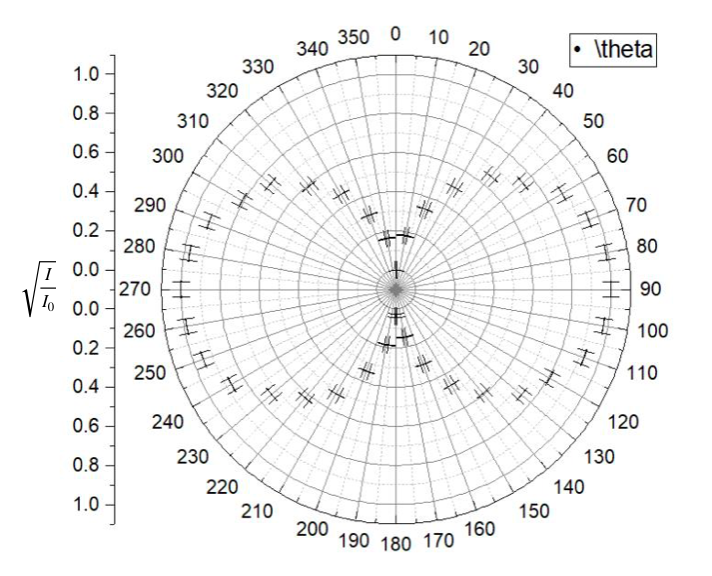
\includegraphics[width=0.7\textwidth]{p1n} 
    \caption{Linear fit for rotation angle 0$^{\circ}$.} 
\end{figure}
\newpage




\subsubsection{\textsc{Rotation angle 20$^\circ$}}
In this section, the data is recorded in Table 8:

\begin{table}[h]
\begin{center}
\begin{tabular}{|c|c|c||c|c|c|}
\hline
\multicolumn{6}{|c|}{Rotation angle of 1/4-wave plate: $20^{\circ}$}\\
\hline 
\multicolumn{6}{|c|}{Maximum Electric Current $I_0$ ~~~ 1.201 $\pm$ 0.001$\mu A$}\\
\hline 
$\theta$ & $I [\mu A] \pm 0.001 [\mu A]$ & $\sqrt{\frac{I}{I_0}}$ & $\theta$ & $I [\mu A] \pm 0.001 [\mu A]$ & $\sqrt{\frac{I}{I_0}}$ \\
\hline
0$^{\circ}$ & 0.156 & 0.3604 & 180$^{\circ}$ & 0.165 & 0.3707 \\
\hline 
10$^{\circ}$ & 0.203 & 0.4111 & 190$^{\circ}$ & 0.234 & 0.4414\\
\hline
20$^{\circ}$ & 0.342 & 0.5336 & 200$^{\circ}$ & 0.359 & 0.5467\\
\hline
30$^{\circ}$ & 0.441 & 0.6060 & 210$^{\circ}$ & 0.483 & 0.6342\\
\hline
40$^{\circ}$ & 0.600 & 0.7068 & 220$^{\circ}$ & 0.641 & 0.7306\\
\hline
50$^{\circ}$ & 0.757 & 0.7939 & 230$^{\circ}$ & 0.792 & 0.8121\\
\hline
60$^{\circ}$ & 0.899 & 0.8652 & 240$^{\circ}$ & 0.923 & 0.8767\\
\hline
70$^{\circ}$ & 1.013 & 0.9184 & 250$^{\circ}$ & 1.051 & 0.9355\\
\hline
80$^{\circ}$ & 1.097 & 0.9557 & 260$^{\circ}$ & 1.140 & 0.9743\\
\hline
90$^{\circ}$ & 1.176 & 0.9895 & 270$^{\circ}$ & 1.201 & 1.0000\\
\hline
100$^{\circ}$ & 1.098 & 0.9562 & 280$^{\circ}$ & 1.152 & 0.9794\\
\hline
110$^{\circ}$ & 0.923 & 0.8767 & 290$^{\circ}$ & 0.971 & 0.8992\\
\hline
120$^{\circ}$ & 0.765 & 0.7981 & 300$^{\circ}$ & 0.821 & 0.8268\\
\hline
130$^{\circ}$ & 0.591 & 0.7015 & 310$^{\circ}$ & 0.620 & 0.7185\\
\hline
140$^{\circ}$ & 0.422 & 0.5928 & 320$^{\circ}$ & 0.462 & 0.6202\\
\hline
150$^{\circ}$ & 0.278 & 0.4811 & 330$^{\circ}$ & 0.289 & 0.4905\\
\hline
160$^{\circ}$ & 0.193 & 0.4009 & 340$^{\circ}$ & 0.231 & 0.4386\\
\hline
170$^{\circ}$ & 0.148 & 0.3510 & 350$^{\circ}$ & 0.162 & 0.3673\\
\hline
\end{tabular}
\caption{Measurement data for the 1/4-wave plate (Rotation angle 20$^{\circ}$).}
\end{center}
\end{table}

In order to calculate $\displaystyle \sqrt{\frac{I}{I_0}}$, we take the case when $\theta = 10^{\circ}$ as a sample calculation, and we will have:
\begin{center}
$\displaystyle \sqrt{\frac{I}{I_0}} = \sqrt{\frac{0.203}{1.201}} = 0.4111 \pm 0.0010$
\end{center}

with relative uncertainty $\displaystyle r = 0.2\% $,which is acceptable. The detailed step for uncertainty calculations are shown in A.3.2.

\newpage
\par Then, we are able to perform a linear fit in polar coordinates with the help of Origin. The result is shown in Fig.10. It can be observed that the transmitted light is elliptically polarized.

\begin{figure}[htb] 
    \centering
    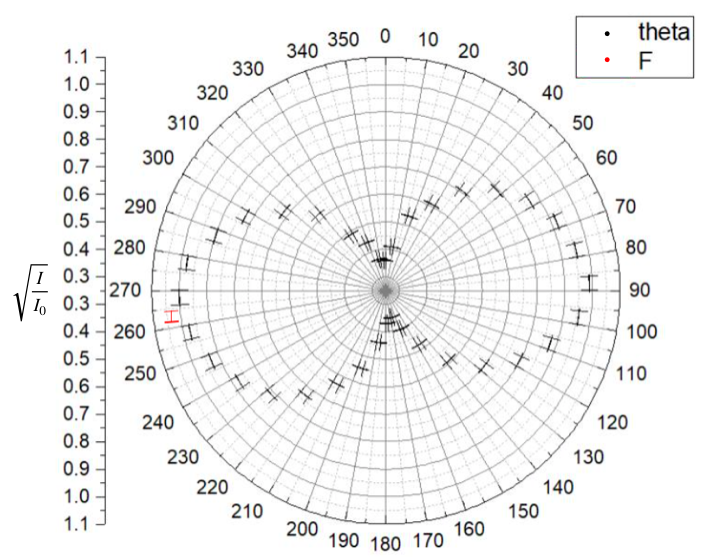
\includegraphics[width=0.7\textwidth]{p2n} 
    \caption{Linear fit for rotation angle 20$^{\circ}$.} 
\end{figure}
\newpage






\subsubsection{\textsc{Rotation angle 45$^\circ$}}
In this section, the data is recorded in Table 9:

\begin{table}[h]
\begin{center}
\begin{tabular}{|c|c|c||c|c|c|}
\hline
\multicolumn{6}{|c|}{Rotation angle of 1/4-wave plate: $45^{\circ}$}\\
\hline 
\multicolumn{6}{|c|}{Maximum Electric Current $I_0$ ~~~ 0.705 $\pm$ 0.001$\mu A$}\\
\hline 
$\theta$ & $I [\mu A] \pm 0.001 [\mu A]$ & $\sqrt{\frac{I}{I_0}}$ & $\theta$ & $I [\mu A] \pm 0.001 [\mu A]$ & $\sqrt{\frac{I}{I_0}}$ \\
\hline
0$^{\circ}$ & 0.612 & 0.9317 & 180$^{\circ}$ & 0.9438 & 0.3707 \\
\hline 
10$^{\circ}$ & 0.629 & 0.9446 & 190$^{\circ}$ & 0.9400 & 0.4414\\
\hline
20$^{\circ}$ & 0.623 & 0.9400 & 200$^{\circ}$ & 0.9416 & 0.5467\\
\hline
30$^{\circ}$ & 0.634 & 0.9483 & 210$^{\circ}$ & 0.9506 & 0.6342\\
\hline
40$^{\circ}$ & 0.650 & 0.9602 & 220$^{\circ}$ & 0.9617 & 0.7306\\
\hline
50$^{\circ}$ & 0.673 & 0.9770 & 230$^{\circ}$ & 0.9785 & 0.8121\\
\hline
60$^{\circ}$ & 0.692 & 0.9907 & 240$^{\circ}$ & 0.9893 & 0.8767\\
\hline
70$^{\circ}$ & 0.681 & 0.9828 & 250$^{\circ}$ & 1.0000 & 0.9355\\
\hline
80$^{\circ}$ & 0.692 & 0.9907 & 260$^{\circ}$ & 0.9957 & 0.9743\\
\hline
90$^{\circ}$ & 0.686 & 0.9864 & 270$^{\circ}$ & 0.9950 & 1.0000\\
\hline
100$^{\circ}$ & 0.685 & 0.9857 & 280$^{\circ}$ & 0.9843 & 0.9794\\
\hline
110$^{\circ}$ & 0.680 & 0.9821 & 290$^{\circ}$ & 0.9763 & 0.8992\\
\hline
120$^{\circ}$ & 0.675 & 0.9885 & 300$^{\circ}$ & 0.9734 & 0.8268\\
\hline
130$^{\circ}$ & 0.661 & 0.9683 & 310$^{\circ}$ & 0.9668 & 0.7185\\
\hline
140$^{\circ}$ & 0.649 & 0.9595 & 320$^{\circ}$ & 0.9572 & 0.6202\\
\hline
150$^{\circ}$ & 0.628 & 0.9438 & 330$^{\circ}$ & 0.9438 & 0.4905\\
\hline
160$^{\circ}$ & 0.620 & 0.9378 & 340$^{\circ}$ & 0.9355 & 0.4386\\
\hline
170$^{\circ}$ & 0.615 & 0.9340 & 350$^{\circ}$ & 0.9378 & 0.3673\\
\hline
\end{tabular}
\caption{Measurement data for the 1/4-wave plate (Rotation angle 45$^{\circ}$).}
\end{center}
\end{table}

In order to calculate $\displaystyle \sqrt{\frac{I}{I_0}}$, we take the case when $\theta = 10^{\circ}$ as a sample calculation, and we will have:
\begin{center}
$\displaystyle \sqrt{\frac{I}{I_0}} = \sqrt{\frac{0.629}{0.705}} = 0.9446 \pm 0.0010$
\end{center}

with relative uncertainty $\displaystyle r = 0.11\% $,which is acceptable. The detailed step for uncertainty calculations are shown in A.3.3.

\newpage
\par Then, we are able to perform a linear fit in polar coordinates with the help of Origin. The result is shown in Fig.11. It can be observed that the transmitted light is circularly polarized.
\par Also, we apply a linear fit to the plot. We find that the value of Pearson's R is 0.02402, and Adj. R-Square is -0.02882. However, the curve is not a perfect circle. We will discuss this phenomenon later.

\begin{figure}[htb] 
    \centering
    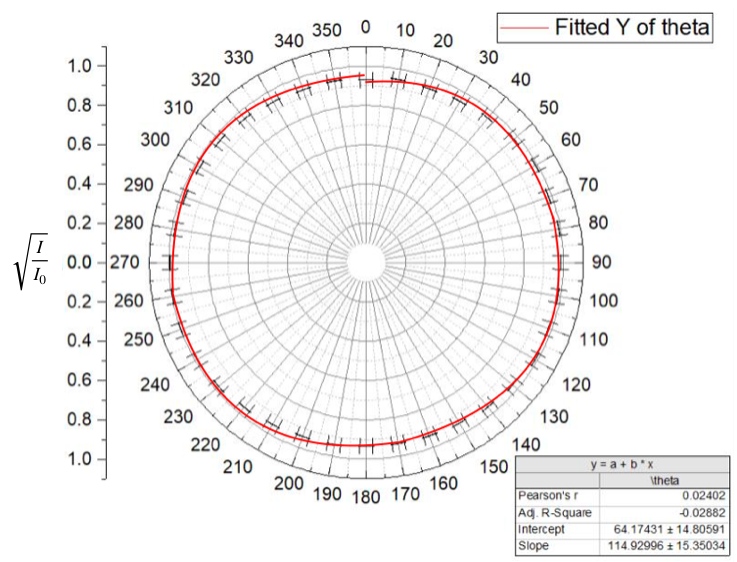
\includegraphics[width=0.7\textwidth]{p3n} 
    \caption{Linear fit for rotation angle 0$^{\circ}$.} 
\end{figure}

\newpage
\subsubsection{\textsc{Rotation angle 70$^\circ$}}
In this part, we rotate the analyzer, and find the position where the light intensity reaches a maximum. The data has been recorded in Table 10.

\begin{table}[h]
\begin{center}
\begin{tabular}{|c|c|}
\hline
\multicolumn{2}{|c|}{Rotation angle of 1/4-wave plate: $70^{\circ}$}\\
\hline 
$\theta$[$^{\circ}$] $\pm$ 2[$^{\circ}$] & 268 \\
\hline 
$I [\mu A] \pm 0.001 [\mu A]$ & 1.221 \\
\hline
\end{tabular}
\caption{Measurement data for the 1/4-wave plate (Rotation angle 45$^{\circ}$).}
\end{center}
\end{table}

\par In section 5.4.2, we have marked the point as "F" in Fig.10 in red.


%----------------------------------------------------------------------------------------
%	SECTION 6
%----------------------------------------------------------------------------------------
\newpage
\section{\textsc{Conclusion and Discussion}}
\subsection{\textsc{Answer to the questions in lab manual}}
\begin{itemize}
\item When the 1/2-wave plate rotates for 360$^{\circ}$, \textbf{4} times of light extinction can be observed.
\item When the analyzer rotates for 360$^{\circ}$, \textbf{2} times of light extinction can be observed.
\item The polarization state won't change. Namely, the transmitted light is still linearly polarized. This is because the function of the 1/2-wave plate is simply to make the polarization axis rotated by angle $2\alpha$. For example, if $\alpha = 45^{\circ}$, then the polarization axis of the transmitted light is vertical to that of the original light.
\end{itemize}

\subsection{\textsc{Discussion}}
In this lab, generally speaking, we do a great job and have some satisfactory results. We verify Malus' Law, and focus on the properties of 1/2 and 1/4-wave plates. The uncertainty is not so large. However, there still exists some errors, like the polar linear fit has a smaller Pearson's r. Hence, some possible sources that may lead to errors are listed below: 
\begin{itemize}
\item Although when doing this lab, we are in a dark environment, light from other groups may disturb us and influence our results.
\item When doing the lab, readings on the digital meter "oscillate" for a long time. In other words, it's hard for the digital meter to be in a steady to ensure an accurate value.
\item The polarizer and analyzer may not be parallel in a line with each other, leading to deviation in refraction.
\item The polarizer's neck is not tight enough, which can be rotated for for some small angle.  
\item Sometimes in this lab, because of darkness, we may misread some value, or rotate the polarizer unintentionally.
\end{itemize}
Based on the above factors and my own thoughts, some suggestions to improve the results are listed below:
\begin{itemize}
\item We can add some window shade between each group so that the light emitted from one group will not influence another group.
\item The design of the polarizer can be modified. To be more specific, a buckle can be added on the polarizer to prevent it from rotating when we don't rotate it intentionally.
\item For oscillating values on the digital meter, we can choose the value in the middle, or we can wait for a longer time for it to be steady. Also, we can do multiple times of experiment and take their average to minimize the errors.
\item The distance between the polarizer and analyzer should be appropriate. Thus we avoid to have a too large or too small current.
\item For simplicity and accuracy, when rotating the polarizer and analyzer, we should always rotate it in one specific direction. 
\item For some old devices, we can change them into new ones.
\end{itemize}

\subsection{\textsc{Conclusion}}
In this lab, we learned a lot, including:
\begin{itemize}
\item We understand the polarization phenomenon of light.
\item We study and verify Malus' Law.
\item We get familiar with 1/2 and 1/4-wave plate which is important in optical systems.
\item Generate, analyze and identify the linearly polarized, circularly polarized, and elliptically polarized light.
\item Learn how to use UT51 digital universal meter, semiconductor laser, and various useful optical apparatuses.
\end{itemize}
To sum up, in this lab we really learned a lot. Not only do we improve our cooperating skills, but we analyze the data, perform some plots by ourselves as well. Based on these analysis, we discuss about the result of the experiment and put forward some suggestions that may help the experiment to be better.
%----------------------------------------------------------------------------------------
%	SECTION 7
%----------------------------------------------------------------------------------------

\begin{appendices} 
\section{\textsc{Measurement uncertainty analysis}} 
	\subsection{\textsc{Demonstration of Malus’ Law}}
	In this section, we record data as shown in Table 3. We want to calculate the uncertainty for $I/I_0$ and $cos^2\theta$. The calculations will shown as follows:
	\begin{itemize}
	\item[(1)] The uncertainty of $I/I_0$ can be obtained through the following formula:
	\begin{center}
	$\displaystyle u_{I/I_0} = \sqrt{(\frac{I}{I_0^2})^2~u_{I_0}^2 + (\frac{1}{I_0})^2 ~ u_I^2}  $
	\end{center}
	Take $\theta = 5^{\circ}$ as a sample calculation, we are able to obtain the uncertainty accordingly:
	\begin{center}
	$\displaystyle u_{I/I_0} = \sqrt{(\frac{1.203}{1.211^2})^2~0.001^2 + (\frac{1}{1.211})^2 ~ 0.001^2} = 0.0012 $
	\end{center}
	with relative uncertainty:
	\begin{center}
	$ \displaystyle r_{u_{I/I_0}} =\frac{u_{I/I_0}}{I/I_0} \times 100\% = 0.12\% $
	\end{center}
	
	Then, all the uncertainties are given in the following Table:
	\begin{table}[h]
	\begin{center}
	\begin{tabular}{|c|c|c|c||c|c|c|c|}
	\hline
	$\theta$ & $I / I_0$ & $u_{I / I_0}$ & $r_{u_{I / I_0}}$ & $\theta$ & $I / I_0$ &  $u_{I / 	I_0}$ & $r_{u_{I / 	I_0}}$\\
	\hline
	$0^{\circ}$ & 1.0000 & 0.0012 & 0.12$\%$ & $50^{\circ}$ & 0.4178 & 0.0009 & 0.2$\%$\\
	\hline 
	$5^{\circ}$ & 0.9934 & 0.0012 & 0.12$\%$ & $55^{\circ}$ & 0.3493 & 0.0009 & 0.3$\%$\\
	\hline 
	$10^{\circ}$ & 0.9727 & 0.0012 & 0.12$\%$ & $60^{\circ}$ & 0.2642 & 0.0009 & 0.3$\%$\\
	\hline 
	$15^{\circ}$ & 0.9265 & 0.0011 & 0.12$\%$ & $65^{\circ}$ & 0.1841 & 0.0008 & 0.4$\%$\\
	\hline 
	$20^{\circ}$ & 0.9273 & 0.0011 & 0.12$\%$ & $70^{\circ}$ & 0.1272 & 0.0008 & 0.6$\%$\\
	\hline 
	$25^{\circ}$ & 0.8720 & 0.0011 & 0.13$\%$ & $75^{\circ}$ & 0.0735 & 0.0008 & 1.1$\%$\\
	\hline 
	$30^{\circ}$ & 0.7853 & 0.0010 & 0.13$\%$ & $80^{\circ}$ & 0.0339 & 0.0008 & 2$\%$\\
	\hline 
	$35^{\circ}$ & 0.7060 & 0.0010 & 0.14$\%$ & $85^{\circ}$ & 0.0107 & 0.0008 & 7$\%$\\
	\hline 
	$40^{\circ}$ & 0.6078 & 0.0009 & 0.15$\%$ & $90^{\circ}$ & 0.0000 & 0.0008 & / \\
	\hline 
	$45^{\circ}$ & 0.5120 & 0.0009 & 0.18$\%$ &  &  &  &   \\
	\hline 
	\end{tabular}
	\caption{Uncertainty of $I/I_0$.}
	\end{center}
	\end{table}
	
	\item[(2)] The uncertainty of $cos^2\theta$ can be obtained through the following formula:
	\begin{center}
	$\displaystyle u_{cos^2\theta} = \sqrt{(\frac{\partial cos^2\theta}{\partial \theta})^2 ~ u_{\theta}^2} = 2sin\theta cos\theta u_{\theta}  $
	\end{center}
	Take $\theta = 5^{\circ}$ as a sample calculation, we are able to obtain the uncertainty accordingly:
	\begin{center}
	$\displaystyle u_{cos^2\theta} = 2sin5^{\circ} cos5^{\circ} \frac{2}{180} \pi = 0.006 $
	\end{center}
	with relative uncertainty:
	\begin{center}
	$ \displaystyle r_{u_{cos^2\theta}} =\frac{u_{cos^2\theta}}{cos^2\theta} \times 100\% = 0.6\% $
	\end{center}
	
	Then, all the uncertainties are given in the following Table:
	\begin{table}[h]
	\begin{center}
	\begin{tabular}{|c|c|c|c||c|c|c|c|}
	\hline
	$\theta$ & $cos^2\theta$ & $u_{cos^2\theta}$ & $r_{u_{cos^2\theta}}$ & $\theta$ & $cos^2\theta$ & $u_{cos^2\theta}$ & $r_{u_{cos^2\theta}}$ \\
	\hline
	$0^{\circ}$ & 1 & 0 & 0 & $50^{\circ}$ & 0.41 & 0.03 & 7$\%$\\
	\hline 
	$5^{\circ}$ & 0.992 & 0.006 & 0.6$\%$ & $55^{\circ}$ & 0.33 & 0.03 & 9$\%$\\
	\hline 
	$10^{\circ}$ & 0.970 & 0.012 & 1.2$\%$ & $60^{\circ}$ & 0.25 & 0.03 & 12$\%$\\
	\hline 
	$15^{\circ}$ & 0.933 & 0.017 & 1.8$\%$ & $65^{\circ}$ & 0.18 & 0.03 & 17$\%$\\
	\hline 
	$20^{\circ}$ & 0.88 & 0.02 & 2$\%$ & $70^{\circ}$ & 0.12 & 0.02 & 17$\%$\\
	\hline 
	$25^{\circ}$ & 0.82 & 0.03 & 4$\%$ & $75^{\circ}$ & 0.067 & 0.017 & 25$\%$\\
	\hline 
	$30^{\circ}$ & 0.75 & 0.03 & 4$\%$ & $80^{\circ}$ & 0.030 & 0.012 & 40$\%$\\
	\hline 
	$35^{\circ}$ & 0.67 & 0.03 & 4$\%$ & $85^{\circ}$ & 0.008 & 0.006 & 75$\%$\\
	\hline 
	$40^{\circ}$ & 0.59 & 0.03 & 5$\%$ & $90^{\circ}$ & 0 & 0 & /\\
	\hline 
	$45^{\circ}$ & 0.50 & 0.03 & 6$\%$ &  &  & & \\
	\hline 
	\end{tabular}
	\caption{Uncertainty of $cos^2\theta$.}
	\end{center}
	\end{table}
	\end{itemize}
	
	\subsection{\textsc{LINEARLY POLARIZED LIGHT AND THE HALF-WAVE PLATE}}
	In this section, for the left column (Rotation angle of the 1/2-wave plate), since it is measured directly without calculations, what we need to consider is only the type-B uncertainty, i.e.
	\begin{center}
	$u_{\theta_1} = u_{\Delta_B} = 2^{\circ}$
	\end{center}
	\par For the right column (Rotation angle of the analyzer), however, it is not the case, since we ought to calculate $\theta_2 = \Delta \theta$, i.e., we have the function:
	\begin{center}
	$\theta_2 = \theta_0 - \theta$
	\end{center}
	Hence the uncertainty can be calculated as:
	\begin{center}
	$\displaystyle u_{\theta_2} = \sqrt{(\frac{\partial \theta_2}{\partial \theta_0})^2~(u_{\theta_0})^2 + (\frac{\partial \theta_2}{\partial \theta})^2~(u_{\theta})^2} = \sqrt{(u_{\theta_0})^2 + (u_{\theta})^2} = \sqrt{2^2+2^2} \approx 3 ^{\circ}$
	\end{center}
	
	\subsection{\textsc{Circularly and Elliptically Polarized Light and the 1/4-wave Plate}}
	Since $f(I,I_0) = \sqrt{I/I_0}$, we are able to find out its uncertainty through the following formula:
	\begin{center}
	$ \displaystyle u_{\sqrt{\frac{I}{I_0}}} = \sqrt{(\frac{\partial f}{\partial I})^2(u_I)^2 + (\frac{\partial f}{\partial I_0})^2(u_{I_0})^2} = \sqrt{\frac{1}{4II_0}~u_I^2 + \frac{I}{4I_0^3}~u_{I_0}^2}$
	\end{center}
	\par By the formula above, we are able to calculate all the uncertainties. Here we take the case when I = 0.047 $\mu A$ with $I_0$ = 1.452 $\mu A$ as an example. The uncertainties can be calculated as:
	\begin{center}
	$\displaystyle u_{\sqrt{\frac{I}{I_0}}} = \sqrt{\frac{1}{4\times0.047\times1.452}\times0.001^2 + \frac{0.047}{4\times1.452^3}\times0.001^2} = 0.002 \mu A$
	\end{center}
	\par Now, all the uncertainties in this part can be calculated similarly.
	
	\newpage
	\subsubsection{\textsc{Rotation angle 0$^\circ$}}
\begin{table}[h]
\begin{center}
\begin{tabular}{|c|c|c||c|c|c|}
\hline
\multicolumn{6}{|c|}{Rotation angle of 1/4-wave plate: $0^{\circ}$}\\
\hline 
\multicolumn{6}{|c|}{Maximum Electric Current $I_0$ ~~~ 1.452 $\pm$ 0.001$\mu A$}\\
\hline 
$\theta$ & $\sqrt{\frac{I}{I_0}}$ & $u_{\sqrt{\frac{I}{I_0}}}$ & $\theta$ & $\sqrt{\frac{I}{I_0}}$ & $\sqrt{\frac{I}{I_0}}$ \\
\hline
0$^{\circ}$ & 0 & / & 180$^{\circ}$ & 0.037 & 0.009 \\
\hline 
10$^{\circ}$ & 0.180 & 0.002 & 190$^{\circ}$ & 0.1874 & 0.0018\\
\hline
20$^{\circ}$ & 0.3371 & 0.0010 & 200$^{\circ}$ & 0.3452 & 0.0010\\
\hline
30$^{\circ}$ & 0.5007 & 0.0007 & 210$^{\circ}$ & 0.5163 & 0.0007\\
\hline
40$^{\circ}$ & 0.6550 & 0.0006 & 220$^{\circ}$ & 0.6243 & 0.0006\\
\hline
50$^{\circ}$ & 0.7460 & 0.0005 & 230$^{\circ}$ & 0.7339 & 0.0005\\
\hline
60$^{\circ}$ & 0.8806 & 0.0005 & 240$^{\circ}$ & 0.8724 & 0.0005\\
\hline
70$^{\circ}$ & 0.9473 & 0.0005 & 250$^{\circ}$ & 0.9488 & 0.0005\\
\hline
80$^{\circ}$ & 0.9886 & 0.0005 & 260$^{\circ}$ & 0.9872 & 0.0005\\
\hline
90$^{\circ}$ & 1.0000 & 0.0005 & 270$^{\circ}$ & 0.9997 & 0.0005\\
\hline
100$^{\circ}$ & 0.9760 & 0.0005 & 280$^{\circ}$ & 0.9721 & 0.0005\\
\hline
110$^{\circ}$ & 0.9219 & 0.0005 & 290$^{\circ}$ & 0.9170 & 0.0005\\
\hline
120$^{\circ}$ & 0.8072 & 0.0005 & 300$^{\circ}$ & 0.8093 & 0.0005\\
\hline
130$^{\circ}$ & 0.7376 & 0.0005 & 310$^{\circ}$ & 0.7404 & 0.0005\\
\hline
140$^{\circ}$ & 0.5938 & 0.0006 & 320$^{\circ}$ & 0.5909 & 0.0006\\
\hline
150$^{\circ}$ & 0.4643 & 0.0008 & 330$^{\circ}$ & 0.4621 & 0.0008\\
\hline
160$^{\circ}$ & 0.3083 & 0.0011 & 340$^{\circ}$ & 0.3049 & 0.0011\\
\hline
170$^{\circ}$ & 0.1485 & 0.002 & 350$^{\circ}$ & 0.166 & 0.002\\
\hline
\end{tabular}
\caption{Measurement data for the 1/4-wave plate (Rotation angle 0$^{\circ}$).}
\end{center}
\end{table}
Based on our analysis above, we obtain the uncertainty of $\sqrt{I/I_0}$ when the angle is $0^{\circ}$.


\newpage
\subsubsection{\textsc{Rotation angle 20$^\circ$}}
\begin{table}[h]
\begin{center}
\begin{tabular}{|c|c|c||c|c|c|}
\hline
\multicolumn{6}{|c|}{Rotation angle of 1/4-wave plate: $20^{\circ}$}\\
\hline 
\multicolumn{6}{|c|}{Maximum Electric Current $I_0$ ~~~ 1.201 $\pm$ 0.001$\mu A$}\\
\hline 
$\theta$ & $\sqrt{\frac{I}{I_0}}$ & $u_{\sqrt{\frac{I}{I_0}}}$ & $\theta$ & $\sqrt{\frac{I}{I_0}}$ & $\sqrt{\frac{I}{I_0}}$ \\
\hline
0$^{\circ}$ & 0.3604 & 0.0011 & 180$^{\circ}$ & 0.3707 & 0.0011 \\
\hline 
10$^{\circ}$ & 0.4111 & 0.0010 & 190$^{\circ}$ & 0.4414 & 0.0009\\
\hline
20$^{\circ}$ & 0.5336 & 0.0008 & 200$^{\circ}$ & 0.5467 & 0.0008\\
\hline
30$^{\circ}$ & 0.6060 & 0.0007 & 210$^{\circ}$ & 0.6342 & 0.0007\\
\hline
40$^{\circ}$ & 0.7068 & 0.0007 & 220$^{\circ}$ & 0.7306 & 0.0006\\
\hline
50$^{\circ}$ & 0.7939 & 0.0006 & 230$^{\circ}$ & 0.8121 & 0.0006\\
\hline
60$^{\circ}$ & 0.8652 & 0.0006 & 240$^{\circ}$ & 0.8767 & 0.0006\\
\hline
70$^{\circ}$ & 0.9184 & 0.0006 & 250$^{\circ}$ & 0.9355 & 0.0006\\
\hline
80$^{\circ}$ & 0.9557 & 0.0006 & 260$^{\circ}$ & 0.9743 & 0.0006\\
\hline
90$^{\circ}$ & 0.9895 & 0.0006 & 270$^{\circ}$ & 1.0000 & 0.0006\\
\hline
100$^{\circ}$ & 0.9562 & 0.0006 & 280$^{\circ}$ & 0.9794 & 0.0006\\
\hline
110$^{\circ}$ & 0.8767 & 0.0006 & 290$^{\circ}$ & 0.8992 & 0.0006\\
\hline
120$^{\circ}$ & 0.7981 & 0.0006 & 300$^{\circ}$ & 0.8268 & 0.0006\\
\hline
130$^{\circ}$ & 0.7015 & 0.0006 & 310$^{\circ}$ & 0.7185 & 0.0006\\
\hline
140$^{\circ}$ & 0.5928 & 0.0007 & 320$^{\circ}$ & 0.6202 & 0.0007\\
\hline
150$^{\circ}$ & 0.4811 & 0.0009 & 330$^{\circ}$ & 0.4905 & 0.0009\\
\hline
160$^{\circ}$ & 0.4009 & 0.0011 & 340$^{\circ}$ & 0.4386 & 0.0010\\
\hline
170$^{\circ}$ & 0.3510 & 0.0012 & 350$^{\circ}$ & 0.3673 & 0.0011\\
\hline
\end{tabular}
\caption{Measurement data for the 1/4-wave plate (Rotation angle 20$^{\circ}$).}
\end{center}
\end{table}
Based on our analysis above, we obtain the uncertainty of $\sqrt{I/I_0}$ when the angle is $20^{\circ}$.




\newpage
\subsubsection{\textsc{Rotation angle 45$^\circ$}}
\begin{table}[h]
\begin{center}
\begin{tabular}{|c|c|c||c|c|c|}
\hline
\multicolumn{6}{|c|}{Rotation angle of 1/4-wave plate: $45^{\circ}$}\\
\hline 
\multicolumn{6}{|c|}{Maximum Electric Current $I_0$ ~~~ 0.705 $\pm$ 0.001$\mu A$}\\
\hline 
$\theta$ & $\sqrt{\frac{I}{I_0}}$ & $u_{\sqrt{\frac{I}{I_0}}}$ & $\theta$ & $\sqrt{\frac{I}{I_0}}$ & $\sqrt{\frac{I}{I_0}}$ \\
\hline
0$^{\circ}$ & 0.9317 & 0.0010 & 180$^{\circ}$ & 0.9438 & 0.0010 \\
\hline 
10$^{\circ}$ & 0.9446 & 0.0010 & 190$^{\circ}$ & 0.9400 & 0.0010\\
\hline
20$^{\circ}$ & 0.9400 & 0.0010 & 200$^{\circ}$ & 0.9416 & 0.0010\\
\hline
30$^{\circ}$ & 0.9483 & 0.0010 & 210$^{\circ}$ & 0.9506 & 0.0010\\
\hline
40$^{\circ}$ & 0.9602 & 0.0010 & 220$^{\circ}$ & 0.9617 & 0.0010\\
\hline
50$^{\circ}$ & 0.9770 & 0.0010 & 230$^{\circ}$ & 0.9785 & 0.0010\\
\hline
60$^{\circ}$ & 0.9907 & 0.0010 & 240$^{\circ}$ & 0.9893 & 0.0010\\
\hline
70$^{\circ}$ & 0.9828 & 0.0010 & 250$^{\circ}$ & 1.0000 & 0.0010\\
\hline
80$^{\circ}$ & 0.9907 & 0.0010 & 260$^{\circ}$ & 0.9957 & 0.0010\\
\hline
90$^{\circ}$ & 0.9864 & 0.0010 & 270$^{\circ}$ & 0.9950 & 0.0010\\
\hline
100$^{\circ}$ & 0.9857 & 0.0010 & 280$^{\circ}$ & 0.9843 & 0.0010\\
\hline
110$^{\circ}$ & 0.9821 & 0.0010 & 290$^{\circ}$ & 0.9763 & 0.0010\\
\hline
120$^{\circ}$ & 0.9885 & 0.0010 & 300$^{\circ}$ & 0.9734 & 0.0010\\
\hline
130$^{\circ}$ & 0.9683 & 0.0010 & 310$^{\circ}$ & 0.9668 & 0.0010\\
\hline
140$^{\circ}$ & 0.9595 & 0.0010 & 320$^{\circ}$ & 0.9572 & 0.0010\\
\hline
150$^{\circ}$ & 0.9438 & 0.0010 & 330$^{\circ}$ & 0.9438 & 0.0010\\
\hline
160$^{\circ}$ & 0.9378 & 0.0010 & 340$^{\circ}$ & 0.9355 & 0.0010\\
\hline
170$^{\circ}$ & 0.9340 & 0.0010 & 350$^{\circ}$ & 0.9378 & 0.0010\\
\hline
\end{tabular}
\caption{Measurement data for the 1/4-wave plate (Rotation angle 45$^{\circ}$).}
\end{center}
\end{table}
Based on our analysis above, we obtain the uncertainty of $\sqrt{I/I_0}$ when the angle is $45^{\circ}$.

\subsubsection{\textsc{Rotation angle 70$^\circ$}}
Since both the values are measured directly, the uncertainty is equal to their type-B uncertainty. Namely, we have:
\begin{center}
$ u_{\theta} = 2^{\circ} $\\
$ u_I = 0.001 [\mu A] $
\end{center}


\newpage
\section{\textsc{Data sheet}} 
See the attached data sheet.
\end{appendices} 

%----------------------------------------------------------------------------------------
%	BIBLIOGRAPHY
%----------------------------------------------------------------------------------------

\begin{thebibliography}{9}
\bibitem{labmanual} Krzyzosiak, M. \& VP141 TA Groups.
\textit{Exercise 5 - lab manual [rev 4.3].pdf}. 
2019.
\end{thebibliography}


%----------------------------------------------------------------------------------------


\end{document}
